\documentclass[tikz,border=10pt]{standalone}
\usetikzlibrary{calc}
% Scale from STYLE METRICS (longest side = 8 cm); coordinates are flipped pixel values
\begin{document}
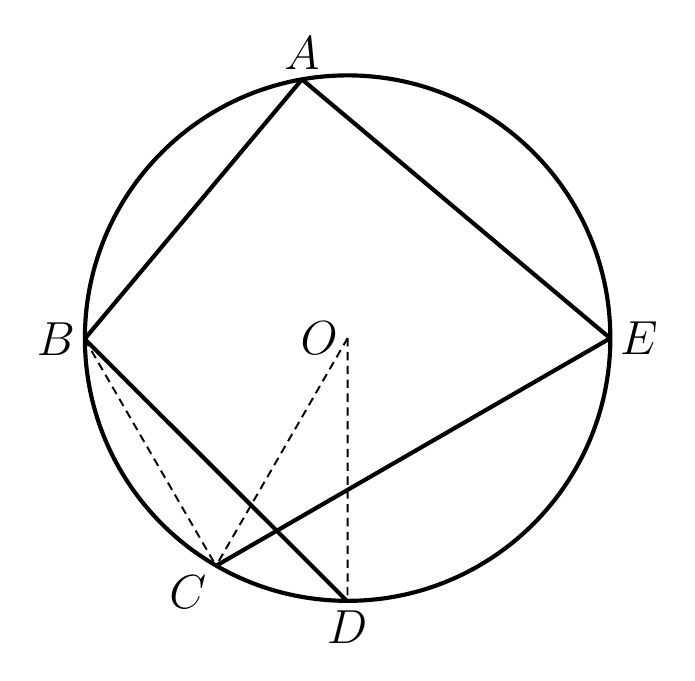
\begin{tikzpicture}[scale=0.02122, line join=round]
  % Points (flipped pixel coordinates)
  \coordinate (O) at (226.0,223.9);
  \coordinate (A) at (198.7,378.7);
  \coordinate (B) at (68.7,223.4);
  \coordinate (C) at (147.3,87.7);
  \coordinate (D) at (225.8,66.5);
  \coordinate (E) at (383.1,223.8);
  % Circle (heavier, solid)
  \draw[line width=1.5pt] (O) circle[radius=157.2];
  % Solid chords (heavier)
  \draw[line width=1.5pt] (A) -- (E);
  \draw[line width=1.5pt] (A) -- (B);
  \draw[line width=1.5pt] (B) -- (D);
  \draw[line width=1.5pt] (E) -- (C);
  % Dashed segments: medium weight, clear dashes (BC, OC, OD only)
  \draw[line width=0.7pt, dash pattern=on 3pt off 2pt] (B) -- (C);
  \draw[line width=0.7pt, dash pattern=on 3pt off 2pt] (O) -- (C);
  % OD: vertical, from O straight down to D (same x as O)
  \draw[line width=0.7pt, dash pattern=on 3pt off 2pt] (O) -- (226.0,66.5);
  % Centre point O: small filled dot
  \fill (O) circle (1.5pt);
  % Labels
  \node[above, font=\fontsize{17}{20.4}\selectfont] at (A) {$A$};
  \node[left, font=\fontsize{17}{20.4}\selectfont] at (B) {$B$};
  \node[below left, font=\fontsize{17}{20.4}\selectfont] at (C) {$C$};
  \node[below, font=\fontsize{17}{20.4}\selectfont] at (D) {$D$};
  \node[right, font=\fontsize{17}{20.4}\selectfont] at (E) {$E$};
  \node[left, font=\fontsize{17}{20.4}\selectfont] at (O) {$O$};
\end{tikzpicture}
\end{document}